\documentclass[11pt, leqno]{article}

%{{{ preamble

\def\doc{The n-Pendulum Problem}
 \def\course{self-study}
\def\abbrev{n-pendulum}
\def\name{A. Mayorov}

%{{{ Preambule

% Some basic packages
\usepackage[T2A]{fontenc}
\usepackage[utf8]{inputenc}
\usepackage[T2A]{fontenc}
\usepackage{textcomp}
\usepackage[russian]{babel}
\usepackage{url}
\usepackage{graphicx}
\usepackage{float}
\usepackage[shortlabels]{enumitem}
\usepackage{csquotes}
\usepackage{changepage}
\usepackage{hyperref}
\usepackage[bottom]{footmisc}
\usepackage{caption}
\usepackage{calc}
\usepackage{geometry}
\geometry{a4paper,bottom=40mm,top=40mm,footskip=20mm}

\usepackage{hyphenat}
\hyphenation{ма-те-ма-ти-ка вос-ста-нав-ли-вать}

% Don't indent paragraphs, leave some space between them
\usepackage{parskip}

% Hide page number when page is empty
\usepackage{emptypage}
\usepackage{subcaption}
\usepackage{multicol}

% Math stuff
\usepackage{amsmath, amsfonts, mathtools, amsthm, amssymb}
\usepackage{xfrac}
% Fancy script capitals
\usepackage{mathrsfs}
\usepackage{cancel}
% Bold math
\usepackage{bm}
% Some shortcuts
\newcommand\N{\ensuremath{\mathbb{N}}}
\newcommand\R{\ensuremath{\mathbb{R}}}
\newcommand\Z{\ensuremath{\mathbb{Z}}}
\renewcommand\O{\ensuremath{\emptyset}}
\newcommand\Q{\ensuremath{\mathbb{Q}}}
\renewcommand\C{\ensuremath{\mathbb{C}}}
\newcommand{\E}{\ensuremath{\mathbb{E}}}  % матожидание
\newcommand{\D}{\ensuremath{\mathsf{D}}}  % дисперсия
\newcommand{\Prb}{\ensuremath{\mathsf{P}}}  % вероятностная мера
\newcommand{\at}{\big\rvert}

\DeclareRobustCommand{\orderof}{\ensuremath{\mathcal{O}}}
\DeclareMathOperator*{\rk}{rk}
\DeclareMathOperator*{\nullity}{Nullity}
\DeclareMathOperator*{\im}{im}
\DeclareMathOperator*{\spn}{span}
\DeclareMathOperator*{\rnk}{rank}
\DeclareMathOperator*{\col}{col}
\DeclareMathOperator*{\row}{row}
\DeclareMathOperator*{\cov}{cov}
\DeclareMathOperator*{\erf}{erf}

\renewcommand{\phi}{\varphi}  % нормальная буква фи
\renewcommand{\le}{\leqslant}  % нормальный знак <=
\renewcommand{\leq}{\leqslant}  % нормальный знак <=
\renewcommand{\ge}{\geqslant}  % нормальный знак >=
\renewcommand{\geq}{\geqslant}  % нормальный знак >=

\DeclarePairedDelimiter\abs{\lvert}{\rvert}%

% Easily typeset systems of equations (French package)
\usepackage{systeme}

% Put x \to \infty below \lim
\let\svlim\lim\def\lim{\svlim\limits}

%Make implies and impliedby shorter
% \let\implies\Rightarrow
% \let\impliedby\Leftarrow
\let\iff\Leftrightarrow
\let\epsilon\varepsilon

% Add \contra symbol to denote contradiction
\usepackage{stmaryrd} % for \lightning
\newcommand\contra{\scalebox{1.5}{$\lightning$}}

% horizontal rule
\newcommand\hr{
    \noindent\rule[0.5ex]{\linewidth}{0.5pt}
}

% Environments
\makeatother
% For box around Definition, Theorem, \ldots
\usepackage{mdframed}

\mdfsetup{skipabove=1em,skipbelow=1em}
\newmdtheoremenv[nobreak=true]{consequence}{Следствие}
\newmdtheoremenv[nobreak=true]{lemma}{Лемма}
\newmdtheoremenv[nobreak=true]{proposition}{Proposition}
\newmdtheoremenv{inference}{Inference}
\newmdtheoremenv{extra}{Extra}
\newmdtheoremenv{problem}{Задача}
\newmdtheoremenv{surmise}{Surmise}
\newmdtheoremenv{observation}{Наблюдение}
\newmdtheoremenv{algorithm}{Алгоритм}
\newmdtheoremenv{application}{Приложение}
\newmdtheoremenv[nobreak=true]{definition}{Определение}

% \theoremstyle{nonumberplain}
\newmdtheoremenv{notation}{Обозначение}
\newmdtheoremenv[ntheorem]{terminology}{Терминология}

\theoremstyle{plain}
\newtheorem*{motivation}{Мотивация}
\newtheorem*{reiteration}{Повторение}
\newtheorem*{interlude}{Interlude}
\newtheorem*{comment}{Комментарий}
\newtheorem*{practice}{Practice}
\newtheorem*{question}{Вопрос}

\newtheoremstyle{example}
  {\topsep}{1em}%
  {}{}%
  {\itshape\bfseries}{\vspace{.5em}\newline}%
  { }{}%

\theoremstyle{example}
\newtheorem{example}{Пример}[section]

\theoremstyle{definition}
\theoremstyle{plain}
\newtheorem*{previouslyseen}{As previously seen}
\newtheorem*{remark}{Замечение}
\newtheorem*{property}{Свойство}
\newtheorem*{intuition}{Интуиция}

\newmdtheoremenv[nobreak=true]{prop}{Proposition}
\newmdtheoremenv[nobreak=true]{theorem}{Теорема}
\newmdtheoremenv[nobreak=true]{corollary}{Corollary}

\makeatletter
  \def\th@definition{
  \thm@headfont{\itshape} % Heading font is italic
  \thm@notefont{}
}
\makeatother

\theoremstyle{definition}
\newtheorem*{solution}{Решение}
\newtheorem*{solution-proof}{Решение}
\theoremstyle{plain}

% End example and intermezzo environments with a small diamond (just like proof
% environments end with a small square)
\usepackage{etoolbox}
\AtEndEnvironment{example}{\null\hfill$\diamond$}%
\AtEndEnvironment{intermezzo}{\null\hfill$\diamond$}%
\AtEndEnvironment{solution}{\null\hfill$\diamond$}%
\AtEndEnvironment{solution-proof}{\null\hfill$\square$}%

\usepackage{titlesec}
\titlespacing*{\section}
{0pt}{5.5ex plus 1ex minus .2ex}{3ex plus .2ex}
\titlespacing*{\subsection}
{0pt}{5.5ex plus 1ex minus .2ex}{4ex plus .2ex}

% Exercise 
% Usage:
% \exercise{5}
% \subexercise{1}
% \subexercise{2}
% \subexercise{3}
% gives
% Exercise 5
%   Subexercise 5.1
%   Subexercise 5.2
%   Subexercise 5.3
\newcommand{\exercise}[1]{%
    \def\@exercise{#1}%
    \subsection*{Exercise #1}
}

\newcommand{\subexercise}[1]{%
    \subsubsection*{Exercise \@oefening.#1}
}

% These are the fancy headers
\usepackage{fancyhdr}
\pagestyle{fancy}

% LE: left even
% RO: right odd
% CE, CO: center even, center odd
% My name for when I print my lecture notes to use for an open book exam.
% \fancyhead[LE,RO]{Gilles Castel}

\fancyhead[L]{\thepage} % Right odd,  Left even
\fancyhead[R]{\name}    % Right even, Left odd
\fancyfoot[L]{}  	 % Right odd,  Left even
\fancyfoot[R]{}          	 % Right even, Left odd
\fancyfoot[C]{}     	 % Center
% \fancyfoot[C]{\leftmark}         % Center
\setlength{\headheight}{14pt}

%\makeatother
%
% Todonotes and inline notes in fancy boxes
\usepackage{todonotes}
\usepackage{tcolorbox}

% Make boxes breakable
\tcbuselibrary{breakable}

\newenvironment{note}[1]{\begin{tcolorbox}[
    arc=0mm,
    colback=white,
    colframe=white!65!black,
    title=#1,
    % fonttitle=\sffamily,
    breakable
]}{\end{tcolorbox}}

% Figure support as explained in Gilles Castel's blog post.
%\usepackage{import}
%\usepackage{xifthen}
%\usepackage{pdfpages}
%\usepackage{transparent}
%\newcommand{\incfig}[2][1]{%
%    \def\svgwidth{#1\textwidth}
%    \import{./figures/}{#2.pdf_tex}
%}
\usepackage{graphicx} %Loading the package
\graphicspath{{figures/}} %Setting the graphicspath

% Quotes
\let\oldquote\quote
\let\endoldquote\endquote
\renewenvironment{quote}[2][]
  {\if\relax\detokenize{#1}\relax
     \def\quoteauthor{#2}%
   \else
     \def\quoteauthor{#2~---~#1}%
   \fi
   \oldquote}
  {\par\nobreak\smallskip\hfill(\quoteauthor)%
   \endoldquote\addvspace{\bigskipamount}}

% Tables
\usepackage[thinlines]{easytable}
\usepackage{booktabs}
\usepackage{xcolor}
\usepackage{hhline}
\usepackage{colortbl}
\usepackage{multirow}
\usepackage{diagbox}

\usepackage{array}   % for \newcolumntype macro
\newcolumntype{L}{>{$}c<{$}} % math-mode version of "l" column type

% Plots
\usepackage{float}
\usepackage{tikz}
\usepackage{pgfplots}

% https://tex.stackexchange.com/questions/149977/how-to-make-invisible-section-header-noticeable-in-the-toc
\makeatletter
\newcommand\invisiblesection[1]{%
  % \refstepcounter{section}%
  \addcontentsline{toc}{section}{\protect\numberline{\thesection}#1}%
  \sectionmark{#1}\phantom{}}
\makeatother

% Code
\usepackage{listings}
\usepackage{xcolor}
\usepackage{mdframed}

\lstset{tabsize=4}
\definecolor{light-gray}{gray}{0.95}

\lstnewenvironment{codefrag}[1]
{\mdframed[backgroundcolor=light-gray, roundcorner=10pt,leftmargin=1,
rightmargin=1, innerleftmargin=15, innertopmargin=10,innerbottommargin=5,
outerlinewidth=1, linecolor=light-gray]\lstset{language=#1}}{
\endmdframed}

%% Fix some stuff
%% http://tex.stackexchange.com/questions/76273/multiple-pdfs-with-page-group-included-in-a-single-page-warning
%%\pdfsuppresswarningpagegroup=1
%
%% My name
\author{Alex Mayorov}


%}}}


% fix some spacing
% http://tex.stackexchange.com/questions/22119/how-can-i-change-the-spacing-before-theorems-with-amsthm

%\makeatletter
%\def\thm@space@setup{%
%\thm@preskip=\parskip \thm@postskip=0pt
%}

%}}}

\usepackage{tikz-qtree}
\usepackage{multirow}
\usepackage{cellspace}
\setlength{\cellspacetoplimit}{0.7em}
\setlength{\cellspacebottomlimit}{0.7em} 

\newtheorem*{note-none}{Замечание}

\usepackage{longtable}
\newcommand{\given}{\;\middle|\;}

\renewcommand{\thesection}{\Alph{section}.}

\begin{document}\thispagestyle{empty}

\begin{center}
	\textbf{\LARGE\doc}\\
	\vspace{.85em}
	\textit{\large Alex Mayorov}
\end{center}
\vspace{1em}

\section{The double pendulum}

I follow the derivation from \href{https://scipython.com/blog/the-double-pendulum/}{here}.

\begin{figure}[H]
        \centering
        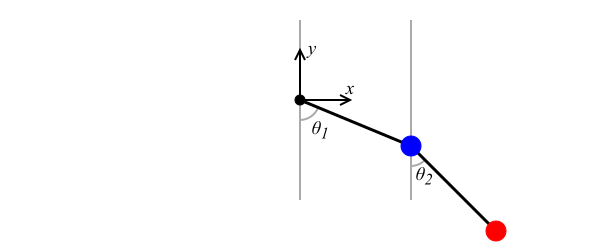
\includegraphics[scale=0.6]{fig/double-pendulum-geometry}
\end{figure}

The two degrees of freedom are $\theta_1$ and $\theta_2$. Then
\begin{align*}
	x_1 &= l_1\sin\theta_1 & \dot x_1 &= l_1 \dot \theta_1 \cos\theta_1 \\
	y_1 &= -l_1 \cos\theta_1 & \dot y_1 &= l_1\dot \theta_1 \sin\theta_1\\
	x_2 &= l_1\sin\theta_1 + l_2\sin\theta_2 & \dot x_2 &= l_1 \dot \theta_1 \cos\theta_1 + l_2 \dot \theta_2 \cos\theta_2\\
	y_2 &= -l_1 \cos\theta_1 - l_2\cos\theta_2 & \dot y_2 &= l_1\dot \theta_1 \sin \theta_1 + l_2 \dot \theta_2 \sin \theta_2
.\end{align*}

Let's compute the Lagrangian, $\mathcal{L} = T - V$:
\begin{align*}
	V ={}& m_1g y_1 + m_2gy_2 \\
	={}& -m_1gl_1\cos\theta_1 - m_2g(l_1\cos\theta_1 + l_2\cos\theta_2) \\
	={}& -(m_1+m_2)gl_1\cos\theta_1-m_2gl_2\cos\theta_2 \\
	T ={}& \frac{1}{2}m_1\dot x_1^2 + \frac{1}{2}m_2\dot x_2^2 + \frac{1}{2}m_1\dot y_1^2 + \frac{1}{2}m_2\dot y_2^2\\
	={}& \frac{1}{2}m_1l_1^2\dot \theta_1^2 + \frac{1}{2}m_2(l_2^2\dot\theta_1^2 + 2l_1l_2\dot\theta_1\dot\theta_2 \cos(\theta_1-\theta_2) + l_2^2\dot\theta_2^2) \\
	={}& \frac{1}{2}(m_1 + m_2)l_1^2\dot \theta_1^2 + \frac{1}{2}m_2l_2^2\dot\theta_2^2 + m_2l_1l_2\dot\theta_1\dot\theta_2\cos(\theta_1-\theta_2) \\
	\mathcal{L} ={}&   \frac{1}{2}(m_1 + m_2)l_1^2\dot \theta_1^2 + \frac{1}{2}m_2l_2^2\dot\theta_2^2 + m_2l_1l_2\dot\theta_1\dot\theta_2\cos(\theta_1-\theta_2) \\
		       &+(m_1+m_2)gl_1\cos\theta_1+m_2gl_2\cos\theta_2
.\end{align*}

We apply the Euler-Lagrange equations, which are:
\begin{equation*}
	\frac{d}{dt}\left( \frac{\partial \mathcal{L}}{\partial \dot q_i} \right)  - \frac{\partial \mathcal{L}}{\partial q_i} = 0\qquad \text{for } q_i = \theta_1, \theta_2 
.\end{equation*}

Therefore,
\begin{align*}
	\frac{\partial \mathcal{L}}{\partial \dot \theta_1} ={}& (m_1 + m_2) l_1^2 \dot \theta_1 + m_2l_1l_2\dot\theta_2\cos(\theta_1 - \theta_2)\\
	\frac{\partial \mathcal{L}}{\partial \theta_1} ={}& -m_2l_1l_2\dot \theta_1\dot \theta_2 \sin(\theta_1-\theta_2) -(m_1+m_2)l_1g \sin\theta_1
\end{align*}
and
\begin{align*}
	&
	\!\begin{multlined}[b]
	 \implies(m_1+m_2)l_1^2\ddot \theta_1 + m_2l_1l_2\ddot \theta_2\cos(\theta_1-\theta_2) - m_2l_1l_2\dot \theta_2\sin(\theta_1-\theta_2)(\dot \theta_1-\dot \theta_2) \\
	= -m_2l_1l_2\dot \theta_1\dot \theta_2\sin(\theta_1-\theta_2) - (m_1+m_2)l_1g\sin\theta_1
	\end{multlined}\\
	&\implies
	(m_1+m_2)l_1\ddot \theta_1 + m_2l_2\ddot \theta_2\cos(\theta_1-\theta_2) + m_2l_2\dot \theta_2^2 \sin(\theta_1-\theta_2) + (m_1+m_2)g\sin\theta_1 = 0
.\end{align*}

Again,
\begin{align*}
	\frac{\partial \mathcal{L}}{\partial \dot \theta_2} ={}& m_2l_2^2\dot \theta_2 + m_2l_1l_2\dot \theta_1\cos(\theta_1-\theta_2) \\
	\frac{\partial \mathcal{L}}{\partial \theta_2} ={}& m_2l_1l_2\dot \theta_1 \dot \theta_2 \sin(\theta_1-\theta_2) - m_2gl_2\sin\theta_2 \\
\end{align*}
and
\begin{align*}
	&\implies m_2l_2\ddot \theta_2 + m_2l_1\ddot \theta_1 \cos(\theta_1-\theta_2) -m_2l_1\dot \theta_1 \sin(\theta_1-\theta_2)(\dot \theta_1 - \dot \theta_2) = m_2l_1\dot \theta_1\dot \theta_2\sin(\theta_1-\theta_2) - m_2g\sin\theta_2\\
	&\implies m_2l_2 \ddot{\theta_2} + m_2l_1 \ddot{\theta_1}\cos(\theta_1-\theta_2)-m_2l_1 \dot{\theta_1^2}\sin(\theta_1-\theta_2) + m_2g\sin\theta_2 = 0
.\end{align*}

Let's introduce $z_1 = \dot{\theta_1}, \dot{z_1} = \ddot{\theta_1}, z_2= \dot{\theta_2}, \dot{z_2} = \ddot{\theta_2}$. This implies

\begin{gather*}
	\begin{cases}
		(m_1+m_2)l_1 \dot{z_1} + m_2l_2 \dot{z_2} \cos(\theta_1-\theta_2) + m_2l_2 z_2^2\sin(\theta_1-\theta_2) + (m_1+m_2)g \sin\theta_1 = 0\\
		m_2l_2 \dot{z_2} + m_2l_1 \dot{z_1}\cos(\theta_1-\theta_2) - m_2l_1z_1^2\sin(\theta_1-\theta_2) + m_2g\sin \theta_2 = 0
	\end{cases}\\ \\
	\begin{cases}
		\begin{split}
			(m_1+m_2)l_1 \dot{z_1} - m_2l_1 \dot{z_1}\cos^2(\theta_1-\theta_2) + m_2l_2 z_2^2\sin(\theta_1-\theta_2) + (m_1+m_2)g\sin\theta_1\\ + m_2l_1z_1^2 \sin(\theta_1-\theta_2)\cos(\theta_1-\theta_2) - m_2g\sin\theta_2\cos(\theta_1-\theta_2) = 0
		\end{split}\\
		\begin{split}
			m_2l_2 \dot{z_2}(m_1+m_2)-m_2l_1z_1^2\sin(\theta_1-\theta_2) (m_1+m_2) +m_2g\sin\theta_2(m_1+m_2) - m_2^2l_2 \dot{z_2} \cos^2(\theta_1-\theta_2) \\ - m_2^2l_2z_2^2\sin(\theta_1-\theta_2) \cos(\theta_1-\theta_2) - (m_1+m_2)m_2g\sin\theta_1\cos(\theta_1-\theta_2) = 0
		\end{split}
	\end{cases}\\ \\
	\begin{cases}
		\dot{z_1} = \frac{m_2g\sin\theta_2\cos(\theta_1-\theta_2) - m_2\sin(\theta_1-\theta_2)[l_1z_1^2\cos(\theta_1-\theta_2) + l_2z_2^2] - (m_1 + m_2)g\sin\theta_1}{l_1[m_1 + m_2\sin^2(\theta_1-\theta_2)]} \\
		\dot{z_2} = \frac{(m_1+m_2)[l_1z_1^2\sin(\theta_1-\theta_2) - g\sin\theta_2  + g\sin\theta_1 \cos(\theta_1-\theta_2)] + m_2l_2z_2^2\sin(\theta_1-\theta_2)\cos(\theta_1-\theta_2)}{l_2[m_1 + m_2\sin^2(\theta_1-\theta_2)]}
	\end{cases}
.\end{gather*}

This forms a system of four first-order ODE in $\dot{z_1}, \dot{\theta_1}, \dot{z_2}, \dot{\theta_2}$ that we can solve numerically, using the Euler or Runge-Kutta method.

\pagebreak
\tableofcontents{}

\end{document}
